%%%%%%%%%%%%%%%%%%%%%%%%%%%%%%%%%%%%%%%%%%%%%%%%%%%%%%%%%%%
% --------------------------------------------------------
% Rho
% LaTeX Template
% Version 1.0 (28/04/2024)
%
% Author: 
% Guillermo Jimenez (memo.notess1@gmail.com)
% 
% License:
% Creative Commons CC BY 4.0
% --------------------------------------------------------
%%%%%%%%%%%%%%%%%%%%%%%%%%%%%%%%%%%%%%%%%%%%%%%%%%%%%%%%%%%
% --------------------------------------------------------
%					  FOR SPANISH BABEL
% --------------------------------------------------------
% \usepackage[spanish,es-nodecimaldot,es-noindentfirst]{babel}
% --------------------------------------------------------
%%%%%%%%%%%%%%%%%%%%%%%%%%%%%%%%%%%%%%%%%%%%%%%%%%%%%%%%%%%

\documentclass[10pt,a4paper,twocolumn]{rho}
\usepackage[english]{babel}
\usepackage{rhoenvs}
\usepackage{multicol}
\usepackage{indentfirst}


%----------------------------------------------------------
% TITLE
%----------------------------------------------------------

\title{Music between the Lines\\On the Heinean Irony in the Song Cycle \textit{Dichterliebe} by Robert Schumann}
%----------------------------------------------------------
% AUTHORS AND AFFILIATIONS
%----------------------------------------------------------

\author{\centering{Henry Lin(Fangheng Lin), \textit{Computer Science and Financial Engineering, Nanjing University}}}


%----------------------------------------------------------
\affil{231275040@smail.nju.edu.cn}
%----------------------------------------------------------
% DATES
%----------------------------------------------------------

%----------------------------------------------------------
% FOOTER INFORMATION
%----------------------------------------------------------
\smalltitle{}
\etal{231275040 \textbf{Lin Fangheng}}
\footinfo{ }
\institution{Nanjing University}
\date{\today}

%----------------------------------------------------------
% ARTICLE INFORMATION
%----------------------------------------------------------

\email{\\
\quad QQ: 3351397126@qq.com\\
\quad Gmail: linhenry980@gmail.com\\
\quad NJU mail: 231275040@smail.nju.edu.cn}
\license{Henry Lin \ccLogo \ student id: 231275040}

%----------------------------------------------------------
% ABSTRACT
%----------------------------------------------------------
\setlength{\parindent}{4ex}

\begin{abstract}
\quad Heinrich Heine, as a renowned German poet and writer, has always been a popular subject of literary research. However, another aspect of Heine's identity, often overlooked (especially domestically), is a lyricist. Schumann, as an important composer of German romanticism, had a deep connection with literature, who was even engaged in literary creation himself. This essay aims to start from the dual identities of Heine and Schumann, using Schumann's \textit{"Dichterliebe,"(A Poet's Love)} based on Heine's \textit{"Buch der Lieder"(Book of Songs),} as the research object. It selects "Heinean irony" as the connecting point for textual and musical analyses, attempting to prove that the "ironic" elements in Heine's original poems are reproduced in different forms in Schumann's music, achieving a perfect fusion of texts and music in this song cycle.
\end{abstract}


%----------------------------------------------------------

\keywords{\textit{Dichterliebe}, Heinrich Heine, Robert Schumann, literature-music relations}

%----------------------------------------------------------
\geometry{left=1.7cm, right=1.7cm, top=1.5cm, bottom=2cm}
\begin{document}
	
    

    \maketitle
    \small{\tableofcontents}
    \thispagestyle{firststyle}
    
    % \tableofcontents

%----------------------------------------------------------

\section*{Writing motivation}
\textcolor{gray}{
 In the upcoming semester, I will be collaborating with my fellow piano club member, Yang Jiahao, to perform Schumann's \textit{Dichterliebe}. To deepen my understanding of this piece and enhance our performance, I have written this essay. By thoroughly analyzing \textit{Dichterliebe} and the concept of "Heinean irony" present within it, I aim to grasp the intricate interplay between music and literature that Schumann masterfully conveys. This analysis helps us accurately interpret the emotional depth and intentions behind the work, thereby enriching our performance and appreciation of this classic composition.}


\newpage
\section*{Overview}
 The essay is divided into five chapters. The first chapter serves as an introduction. The second chapter explains two basic concepts involved in this paper: namely "Kunstlied(art song)" (the genre of \textit{Dichterliebe}) and the definition of "Heinean irony" in the literary domain. In the third chapter, the author introduces Schumann's dual talent in music and literature, as well as the role of literature in his musical creation, followed by a discussion on the common aesthetic points between Schumann and Heine. The forth chapter provides a textual and musical analysis based on two selected songs showing that "Heinean irony" in this song cycle is reflected in the difference between what is said and what is meant. When analyzing the songs, the author first examines the text to identify the ironic elements in Heine's original poems, then points out the modifications Schumann made during the composition process together with their underlying intentions. Following this, the author analyzes the musical reproduction of irony through the choice of keys, rhythm settings, coordination between the vocal and accompaniment parts, as well as the coda's musical figures. The paper concludes that this song cycle is not "overly gentle" as previous studies have suggested, but rather fully expresses the "irony" present in Heine's original poems.

    %\newgeometry{outer=1.7cm, inner=1.7cm, top=1.5cm, bottom=2cm}
    \fancyfootoffset{0pt}
    \onecolumn
    
\section{Introduction}
\rhostart{T}he song cycle \textit{Dichterliebe} made by the romantic composer Robert Schumann is one of the most famous song cycles in music history. Due to its beautiful melody (among other reasons), this masterpiece remains a "regular guest" at concerts. The popularity of the cycle "is likely surpassed only by Schubert's \textit{Winterreise} in Germany, but by no other German song cycles abroad." Moreover, it is also a subject of study because of its high literary quality and musical aesthetics. The text source comes from Heinrich Heine's \textit{Buch der Lied(Book of Songs)} (section \textit{Lyrisches Intermezzo}), a collection of poems and ballads published in 1824, which deals with disappointed love, longing for hope, and simple folk beliefs. As the musicologist Albrecht Dümling notes, the \textit{Buch der Lied} then literally became a book of songs. Some songs, such as\textit{ "The Lorelei,"} became so well-known that people even forgot who originally wrote the lyrics.\textsuperscript{\cite{ref1}}

\section{Conceptual Explanation}
 In this chapter, some fundamental concepts will be explained: the art song and its significance in research concerning the border area between literature and music, as well as Heinean irony with its forms of expression.

\subsection{Kunstlied(Art Song)}
 Lied is a term used in both musicology and literary studies, in which texts and melodies are combined. There are various types of Lied, such as folk songs, hymns, and art songs. The songs discussed below belong to the category of art songs. This genre holds a special place in German romanticism and embodies the ideal of romantic poetics: different art forms unite to form "a new whole of art". Thanks to the contributions of famous composers such as Franz Schubert and Robert Schumann, German poetry has achieved worldwide recognition and remains influential today.

This genre emerged in 1810 with Franz Schubert's compositions, underwent a process of continuous musical transformation over the century, and experienced the end of its heydays in the works of Richard Strauss as well as Arnold Schoenberg. Throughout this process, the focus was on European-language songs. In a broader sense, the art song is a solo song from the Western world with (chordal) instrumental accompaniment since the introduction of monody around 1600. 

The musicologist Hans-Joachim Hinrichsen summarized the characteristics of art songs in his essay \textit{Das Kunstlied als musikalische Lyrik} as follows:\textsuperscript{\cite{ref3}}

\begin{quote}
    \textcolor{darkgray}{"The careful selection of text templates, the idiosyncratic and melodically complex structures that break away from the traditional ideal of simplicity, an autonomously-structured piano accompaniment (with the piano used as the irreplaceable instrument), a sophisticated compositional texture, a structure subtly shifting between strophic form and through-composition, and a harmony extending far beyond mere basic levels."}
\end{quote}

Two points are noteworthy here: the literary quality of the text is important. For example, Schumann set poems by Heine, Uhland, Eichendorff, and Rückert to music. He chose these poets because their poems embodied "the new poetic spirit" and "were reflected in the music." Music, particularly the piano part, does not merely fulfill an accompanying function but plays an equally important role alongside the text. In a certain sense, the musical setting is an interpretation of the text.

\subsection{Heinean Irony}
\indent Heine's work is characterized by the literary device of irony. He once remarked that his poems, even when "the lyrical stands out, are entirely permeated by a more intellectual element, irony." This gives rise to a specific concept: Heinean irony.

Heinean irony is aimed specifically at "the dissolution of unrealistic dreams". Heine's poems are full of contrasts and broken points, and one always encounters "ironic points, the use of banalities, the parody of topoi, and self-irony" in his works. "The moment of contrast" is of great importance to Heine, especially in the context of dream and reality. There are two essential features of Heine's irony: the first feature is a disillusioning function consistent with romantic irony, and the second is the torn nature that repeatedly surfaces in his poems.

Regarding Heine's \textit{Buch der Lieder}, some scholars argue that in this work, "an underlying-skeptical-ironic tone seems to resonate more or less subtly." The ironic placement in poems serves the purpose of "creating distance and ensuring self-protection." Laughter and comedy are part of the "survival strategy of a wounded and torn individual." They are rather a mask and shell of the poet. A detailed explanation of the term with specific examples is provided below along with text analysis.

\section{Schumann's Dual Talent and Turn to Heine's Texts}

In this chapter, Schumann's dual talent in literature and music is first explored. Subsequently, the literary influence on his musical creations and music criticism will be examined. After that, the reason for Schumann's aesthetic approach to Heine and his turn to Heine's texts is explained.

\subsection{Poet or Musician? Schumann's Dual Talent}
Robert Schumann, born on August 6, 1810, and died on July 29, 1856 (the same year Heinrich Heine passed away), is a unique personality in music history. No other composer was as strongly influenced by literary Romanticism as Schumann. To truly understand Schumann's musical works, one must first become acquainted with the literary influences that shaped this young man.

The musicologist Albrecht Dümling expressed it as follows: "Schumann belonged to the artists for whom their dual talent was a genuine dilemma – like Paul Klee between music and painting and Gottfried Keller between painting and literature, the young Schumann wavered between poetry and music." Schumann's inclination towards literature can be traced back to his father, a bookseller from Zwickau. Under his influence, Schumann had access to a very broad spectrum of readings and began creating his own poetry. Already in his youth, Schumann was convinced that poetry and music share the same origin and have the same effect.

Although his literary achievements are not particularly recognized, the literary influence can be found in his musical creations, particularly in the Lied, which is characterized by high literary quality and the equal importance of music and text. Schumann placed great emphasis on the textual basis when setting music, which is why he harshly criticized Schubert for "not paying attention to the quality of his texts" and for "setting the entire German literature to music." Unlike Schubert, Schumann carefully chose the poets for his songs: he set works by Heine, Eichendorff, Goethe, Uhland, Chamisso, Rückert, and Mörike to music.

Schumann's preference for literature is also evident in his instrumental works, such as in the famous piece \textit{Papillons} (Op. 2), which is largely based on Jean Paul's novel \textit{Flegeljahre}. It is indisputable that Schumann was strongly influenced by Jean Paul. As early as 1828, Schumann considered Jean Paul's works to be "works of genius," in which "poetry and music merge." Schumann learned to hear music poetically from this, but also to recognize the limits of language, as it is only confined to what can be said, whereas "music is the wonderful interpreter of the unsayable." Gradually, Schumann turned to music and established his own musical aesthetics. Two philosophical principles of Schumann's musical aesthetics are essentially owed to Jean Paul's influence: "One principle defines music as language, the other conditions speaking about music," which is reflected in Schumann's musical creations and his music-critical essays.

The incompatible sibling pair Walt and Vult from Jean Paul's \textit{Flegeljahre} became the model for the fictional split of Schumann's own self into the doppelgängers Florestan and Eusebius. These are two imaginary figures created by Schumann, forming a pair of opposites that he developed during his career as a music critic. They serve as a central and significant means to express various views of artistic perception. These two fictional figures are also a psychological reflection of Robert Schumann. Florestan represents Schumann's wild side, while Eusebius embodies his gentle side. In his reviews, the two figures engage in dialogues, arguing about the same composer or the same work. Their respective remarks are therefore very different: while Florestan's reviews are more "based on knowledge of the musical text and demonstrate his analytical detail critique," Eusebius tends towards the thought process in music and views music more as a listening experience.

This "fragmentation of the self into two opposing characters" appears not only in Schumann's music criticism but also in his musical compositions and song settings. The "contrasting artistic character" in Schumann's musical aesthetics is, in a certain sense, similar to Heine's literary views and can also be seen as a nexus of Heine's irony. Due to this contradiction and versatility, Schumann could deeply empathize with Heine's sense of fragmentation and point of irony, and he could transfer the ironic elements into his music in his own way. This point will be analyzed in the following.

\subsection{Schumann and Heine: An Encounter}

Heine occupies a special place in Schumann's song compositions. With Heine's texts, "Schumann experienced his breakthrough as a song composer and set a total of 40 of Heine's poems to music." (For comparison, it should be mentioned that the next most frequently set poets are Rückert with 26 poems, Goethe with 19 poems, and Eichendorff with 16 poems.) What made Heine's texts particularly attractive to Schumann, in my opinion, are the biographical similarity and the aesthetic affinity.

First, it is noteworthy that Schumann and Heine met only once, in May 1828. At that time, Schumann was just a high school graduate from Zwickau. Heine had already published \textit{Buch der Lieder} and had made a name for himself. Heine received the young man kindly. After the visit in Munich, Schumann referred to the poet in his diary as "an ironic little man." Subsequently, Schumann engaged intensively with Heine's works, and his admiration for Heine gradually displaced his admiration for Jean Paul. In 1835, Schumann mentioned "four names as examples of great poetry: Shakespeare, Goethe, Schiller, and Heine" in a review.

The main theme of \textit{Buch der Lieder} is unhappy love. There were events in Heine's life that explain this theme: the sorrowful experience with his cousin Amalie. During this time, Robert Schumann fell in love with Clara Wieck but faced strong opposition from Clara's father. Schumann found a resonance in Heine's poetry and identified with the poet due to his own conflict-ridden love story. In 1836, Schumann wrote in a review of Heine settings that they were "an expression of deep, wounded pain." This comment demonstrates his deep understanding of Heine's pain because such pain was very familiar to him as well.

The biographical similarity forms the basis for Schumann's affinity for Heine, but it is only the external reason for it. More importantly, Schumann finds an aesthetic resonance in Heine's poetry. It is not the general theme of love and love's sorrow, but the irony and conflicts inherent in Heine's poetry that particularly attracts this composer. As analyzed above, the sense of being torn apart plays an important role in Schumann's aesthetics. And in Heine's works, Schumann also saw two opposing poles: active optimism and passive, melancholic skepticism, romantic sentiment and disillusioning irony. He found his own contradictions emotional states reflected here.

According to Dümling, this sense of being torn was determined by the era: 

\begin{quote}
\textcolor{darkgray}{"The split between adaptation and resistance, retreat and breakthrough, Biedermeier and Vormärz was characteristic not only for Schumann and Heine, but for the entire Restoration period under Metternich's regime. However, in Schumann and Heine, it particularly emerged as a pronounced conflict."}
\end{quote}

In a certain sense, both of them were inappropriate reactionaries in their era: Schumann, who is generally regarded as a musical Romantic, actually held a contradictory attitude towards the "backward-looking, otherworldly" Romanticism. "I am heartily sick of the word Romantic," he wrote in 1836. A similar observation can be made about Heine. In his early poetry, one can still find romantic traces, but in later years, he sharply criticized Romanticism in his \textit{Romantische Schule}. Heine and Schumann brought German Romanticism to its peak and at the same time paved the way for the breakthrough of European modernity in the bourgeois era."

Returning to \textit{Dichterliebe}, an artistic connection between the poet and the composer, the poet provided Schumann "a framework in which Schumann could express his feelings and simultaneously distance himself from them." Therefore, the musical setting is also considered an interpretation of Heine's works. The music here not only plays a descriptive role but also takes on an illustrative function. This tension between emotional expression and ironic distancing is brilliantly explored by Schumann in all its depth.

\section{Analysis of the Text-Music Relationship in the Song from an Irony Perspective}

In this chapter, one of the categories of Heinean irony is analyzed: the differences between what is said and what is meant. This means that what is said is different from what is meant. The underlying meaning can be explored. The following three poems were selected because irony holds a special place in them. The following questions is considered: How does Heine use this stylistic device? How does it function in the poem? In the musical setting, Schumann more or less processes the text template. What is the intention behind this processing? What is the text-tone relationship like? In what way does Schumann musically interpret these poems?

\subsection{"Ich grolle nicht": Denying as a Mask}
Heine: \textit{Lyrisches Intermezzo XVIII}, Schumann: \textit{Dichterliebe, op. 48/7}
\columnseprule=1pt 
\begin{multicols}{2}

\small {
\noindent Ich grolle nicht, \\
und wenn das Herz auch bricht,\\  
Ewig verlornes Lieb! ich grolle nicht.\\
Wie du auch strahlst in Diamantenpracht,\\
Es fällt kein Strahl in deines Herzens Nacht.\\
Das weiß ich längst.\\
Ich sah dich ja im Traum,\\
Und sah die Nacht in deines Herzens Raum,\\
Und sah die Schlang, die dir am Herzen frißt, \\ 
Ich sah, mein Lieb, wie sehr du elend bist.\\
\columnbreak

\noindent I bear no grudge, \\
even though my heart is breaking, \\ 
Forever lost love! I bear no grudge.  \\
However you may shine in diamond splendor,\\  
No ray of light falls into the night of your heart.  \\
I’ve known that for a long time.\\ 
I saw you in my dreams,\\  
And saw the night within your heart’s space,  \\
And saw the serpent that gnaws at your heart,  \\
I saw, my love, how very miserable you are.}
\end{multicols}
This little poem by Heine was written in the autumn of 1821. It "belongs to the milestones of his early lyrics" and is "characterized by high artistic perfection." The entire poem is a manifesto of the lyrical "Ich(I)" The lyrical "I" claims that it does not bear a grudge, although it lost its beloved and its heart broke as a result, which is an obvious lie. The chosen couplets and the consistently masculine cadences, as well as the unusually long lines in this entire cycle, express strong emotionality.

The irony in this poem is not hard to find, as the repeated assertion "Ich grolle nicht" conceals the bitter feeling. But this is not the only contrast. For example, there is another contrast between the external light ("Diamantenpracht") and the internal darkness ("deines Herzens Nacht") in the third and fourth lines. Heine uses the double meaning of the word "strahlen" here: the ray of diamonds cannot unfortunately bring light to the heart's night. 

"Das weiß ich längst.(I’ve known that for a long time.)" in the second stanza places the reader in a different time frame, namely in a dream. The tense shifts from present to past. The lyrical "I" see the darkness and the snake in the beloved's heart. It feels in the dream that its beloved was very miserable. "The heart's night" can be interpreted differently here. It seems that the beloved is suffering herself, and the snake represents the creeping pain. It is more a deep empathy than a simple lament.

In summary, Heine expresses very complicated feelings in this short eight-line poem. At least four different emotional levels can be identified: \textbf{denial of grudge, expression of lament, empathy with the pain, and finally, possible forgiveness.} All these emotions make the initial assertion "Ich grolle nicht" ironic and ridiculous. It is both a cover-up and a protection. Behind this cover-up lies the broken heart, and with this protection, it can continue to deceive itself.

Schumann's setting is one of the most famous songs in this cycle. Scholars believe that "the song marks a triple peak in the intensity of protest; in the dramaturgy of the cycle; and in Schumann's songwriting." Although Peters understands the text template as a "theme of gradual overcoming of the loss of love" and analyzes the musical design on this basis, which I fundamentally reject, this view is also defensible from my understanding of this song. Schumann manages to translate the irony and the emotional nuances in the text into music.

Schumann does not make any literal changes to the text template here but rearranges the two stanzas: the key phrase "Ich grolle nicht" appears twice in the text template, while Schumann repeats it a total of six times in his setting, each time with an emotional shift. The text looks like this (the parts newly arranged by Schumann are in parentheses):
\begin{quote}
Ich grolle nicht, und wenn das Herz auch bricht,\\  
Ewig verlornes Lieb, (ewig verlornes Lieb!)  \\
ich grolle nicht. (ich grolle nicht.)\\
Wie du auch strahlst in Diamantenpracht,\\
Es fällt kein Strahl in deines Herzens Nacht, (das weiß ich längst.)\\ 
(Ich grolle nicht, und wenn das Herz auch bricht,)\\
Ich sah dich ja im Traum, und sah die Nacht in deines Herzens Raum,\\ 
Und sah die Schlang, die dir am Herzen frißt,  \\
Ich sah, mein Lieb, wie sehr du elend bist.  \\
(Ich grolle nicht, ich grolle nicht.)
\end{quote}

Schumann chooses the simple unembellished key of C major for this song. Schubart himself describes it as a pure key: Innocence, simplicity, naivety, child language are its character. A piece of music composed in this key usually conveys a feeling of confidence and strong will. A famous example is the finale of Beethoven's Fifth Symphony – a heroic movement. This key choice corresponds well with the childish determined key phrase in the text: "Ich grolle nicht." But the actual effect is contradictory. It is "a grotesquely alienated C major." The dissonances and the pounding effect produced by the constant hammering major chords and the triumphant volume sound much more desperate than steadfast, which is "associated with the affect of anger."
\begin{figure}[H]
    \centering
    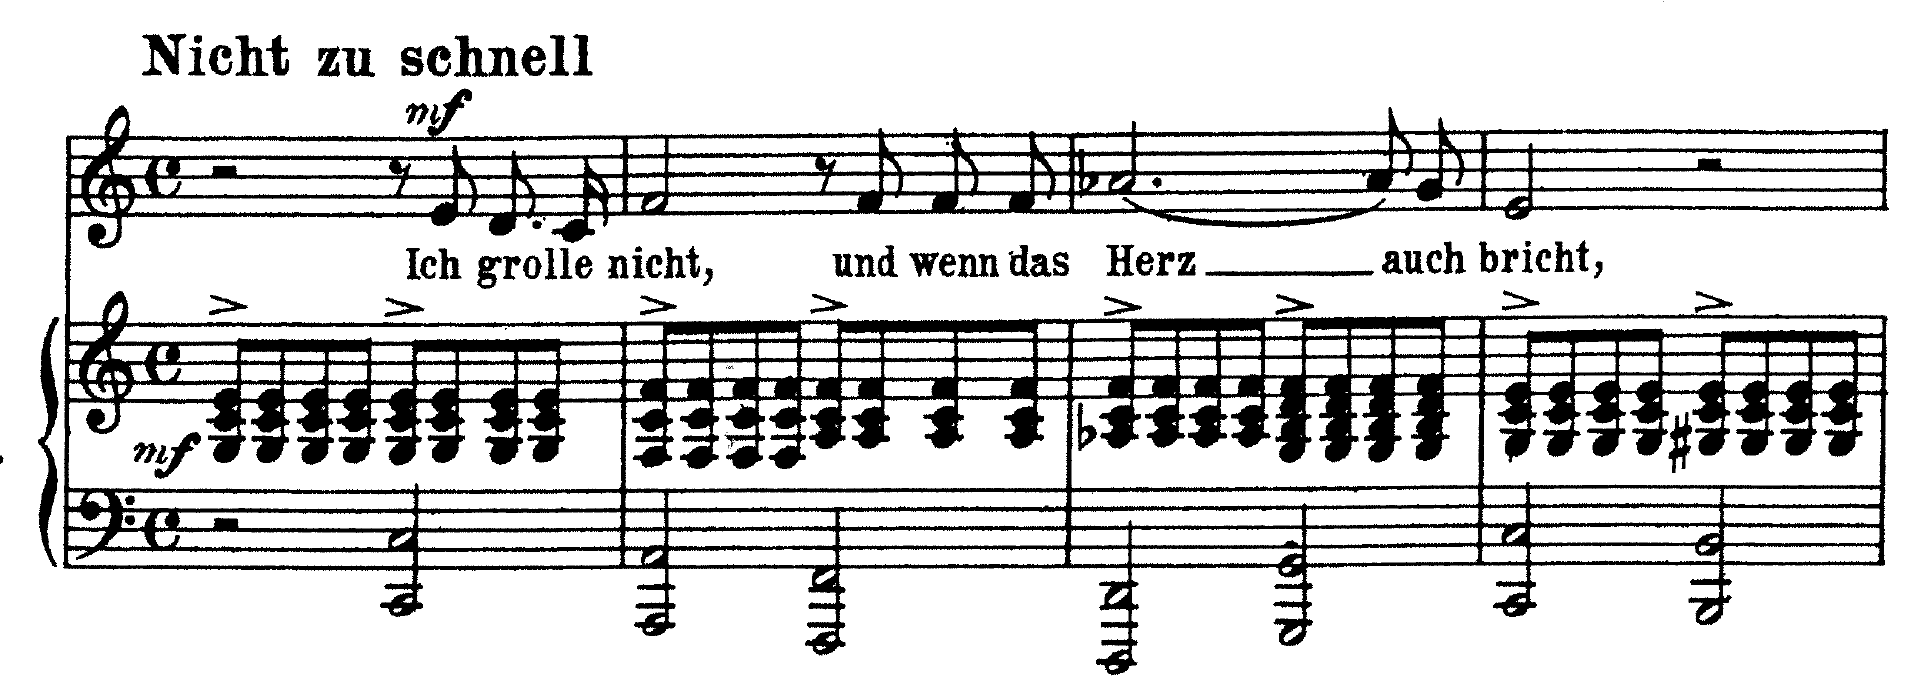
\includegraphics[width=0.7\linewidth]{Ich grolle nicht.png}
    \caption{The Begining of “Ich grolle nicht”}
    \label{“Ich grolle nicht”}
\end{figure}
Already in the text analysis, the four different emotional levels in the poem are mentioned, namely denial of grudge, expression of lament, empathy with the pain, and finally, possible forgiveness. Schumann repeats "Ich grolle nicht" four times in his setting, which in my opinion corresponds to the four emotional shifts. The first two feelings are not hard to identify, but the last two shifts are controversial. However, such a word-tone relationship appears multiple times in this song. Schumann exploits the meaning of the word "längst" and emphasizes it with a crescendo marking for almost one and a half measures, reflecting the long duration and transition to another temporal level, thus representing the second part of the setting (see Figure 2).
\begin{figure}[H]
    \centering
    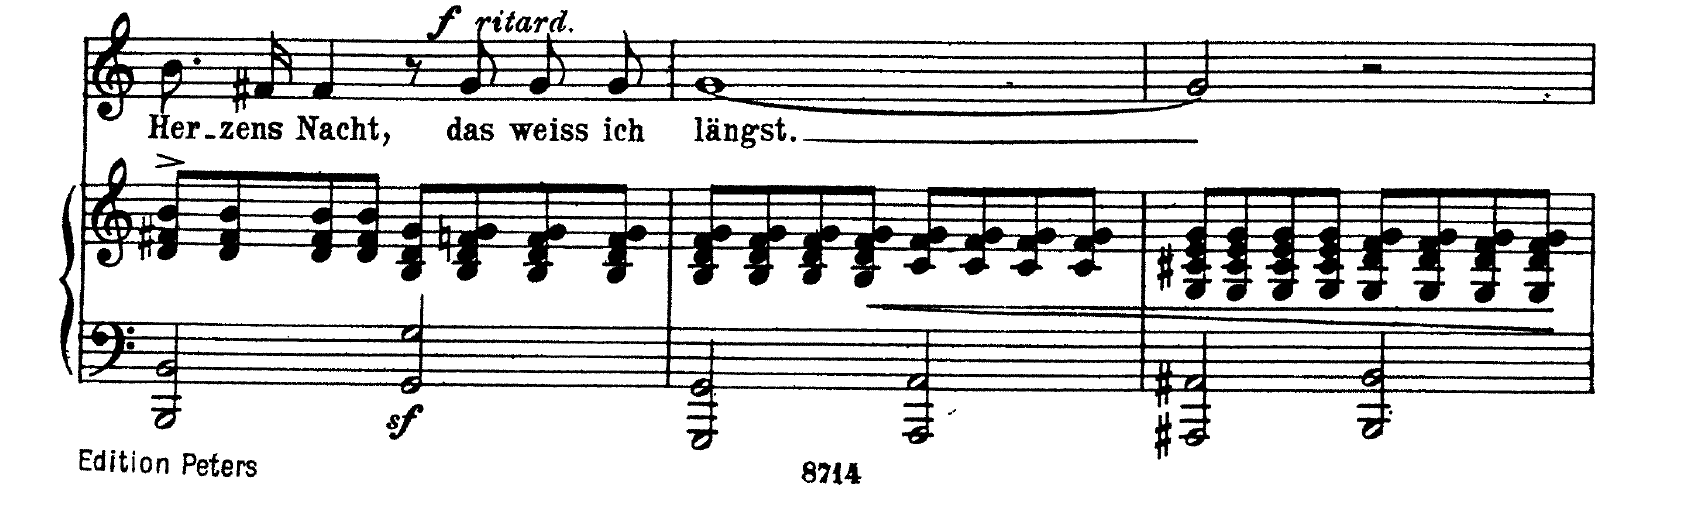
\includegraphics[width=0.7\linewidth]{langst.png}
    \caption{The word "längst"}
    \label{fig:enter-label}
\end{figure}
 And with the word "Herzen" in the phrase "sah die Schlang, die dir am Herzen frißt" the song reaches its highest note and accordingly the emotional peak. In this dream phase, there are no dissonances. The repetition of notes is an attempt to empathize with and digest the beloved's feelings. At the last line "Ich sah, mein Lieb, wie sehr du elend bist," the vocal line does not continue upward but descends chromatically. With the tempo mark ritardando and the natural sign, namely at the word "Lieb," grudge and despair disappear. Only forgiveness and love remain (see Figure 3).
\begin{figure}[H]
    \centering
    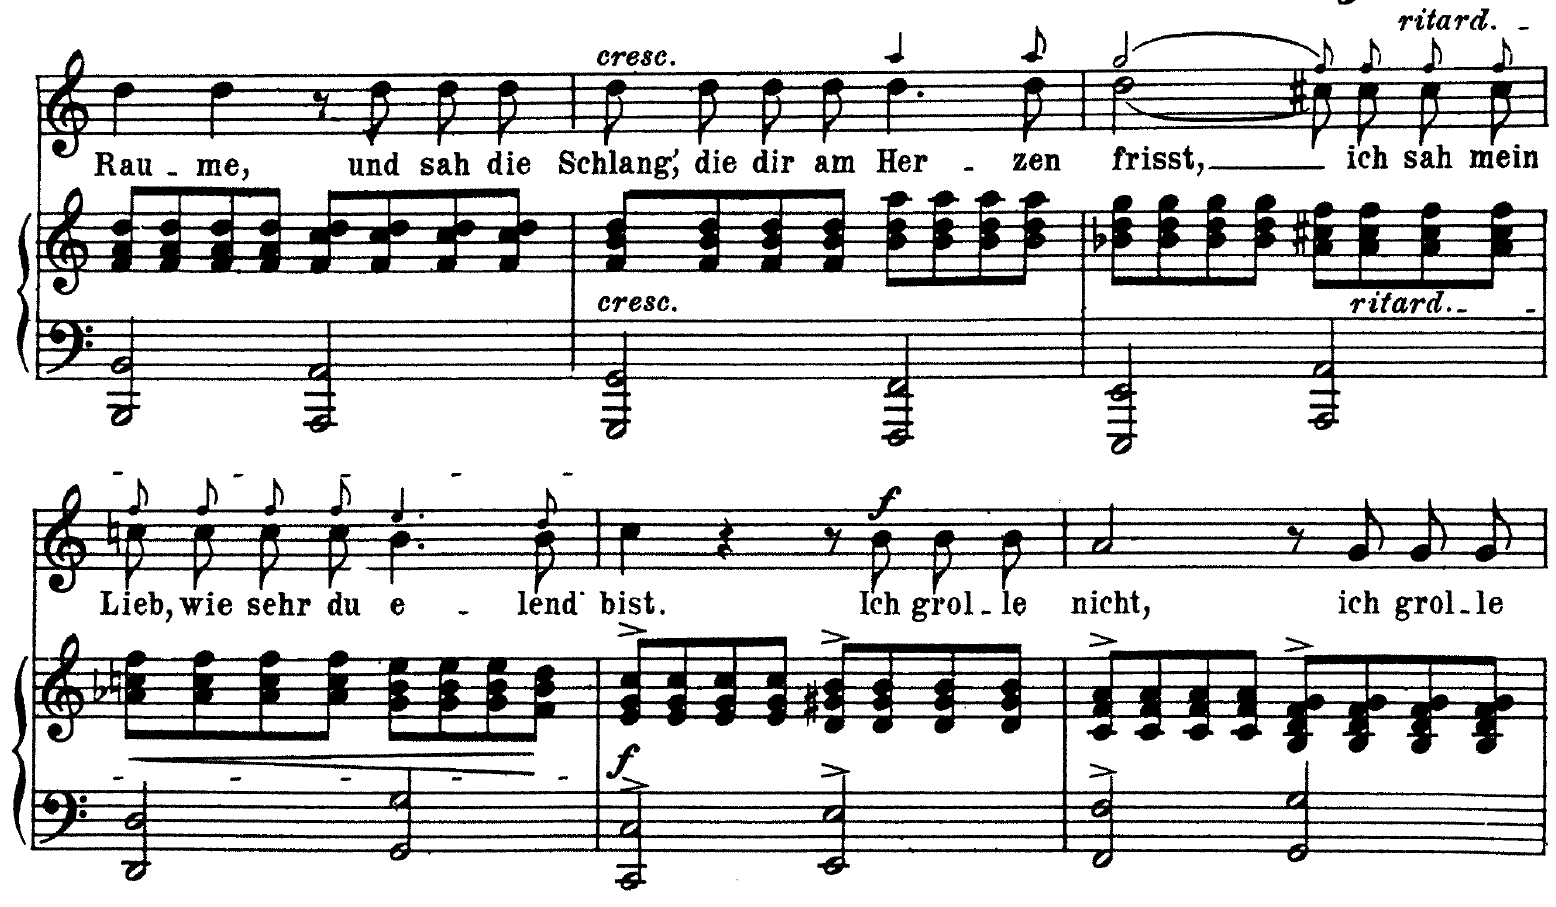
\includegraphics[width=0.7\linewidth]{Herzen and Liebe.png}
    \caption{the word "Herzen" and "Lieb"}
    \label{fig:enter-label}
\end{figure}
In summary, this chapter disproves the view that "Schumann only exposes the superficial irony: the lyrical 'I' bears a grudge." Schumann not only translates Heine's irony and self-protective denial in his setting but also the deep emotional shifts, demonstrating the composer's fine literary sensitivity.

\subsection{"Das ist ein Flöten und Geigen": Objectivity as a Shell}
Heine: \textit{Lyrisches Intermezzo XX}, Schumann: \textit{Dichterliebe, op. 48/9}

\columnseprule=1pt 
\begin{multicols}{2}
\noindent Das ist ein Flöten und Geigen,\\
Trompeten schmettern drein;\\
Da tanzt den Hochzeitreigen\\
Die Herzallerliebste mein.\\
Das ist ein Klingen und Dröhnen,\\
Von Pauken und Schalmei’n;\\
Dazwischen schluchzen und stöhnen\\
Die guten Engelein.

\columnbreak

\noindent There is fluting and fiddling,\\
Trumpets blaring out;\\
There dances the wedding ring\\
My dearest sweetheart.\\
There is a clanging and booming\\
Of drums and shawms;\\
In between, sobbing and groaning\\
The good little angels.

\end{multicols}

This poem was written in the autumn of 1821 and consists of two stanzas, each with four lines. It is composed in iambic trimeter with a cross rhyme scheme and describes the wedding of the "Herzallerliebste" (beloved) of the lyrical "I." This sorrowful situation is described by the lyrical "I" in a cool and detached manner. It does not use emotional and subjective expression but rather provides a straightforward and objective account of the wedding, which, to some extent, appears quite strange within the context of the entire song cycle.

The lyrical "I" seems to feel like an outsider here, hearing merry sounds from various instruments and seeing the wedding dances. Finally, it hears a good angel sobbing and moaning. It is not the lyrical "I" but the angel who weeps over this event. The last two lines form the punchline of the poem. This contrasts sharply with the liveliness and merriment of the wedding. Only with these two brief lines does all the semblance of objectivity and detachment fall apart, revealing the cool observer as a self-deceiver.

However, upon closer reading of the first six lines, something else emerges: "Trompeten schmettern drein" (Trumpets blare out) (line 2), and "Das ist ein Klingen und Dröhnen" (There is a clanging and booming) (line 5) seem to be direct descriptions, but the following two words unmask the poet's facade: "schmettern" (blare) and "dröhnen" (boom). The poet frequently uses these two words to represent a disruptive and not-so-pleasant sound. Moreover, it can be noted that the lyrical "I" almost exclusively uses its sense of hearing, despite actually being at the wedding. There are no detailed descriptions of the wedding itself, only of various sounds. This reduction and restriction to a single sense organ reflect, to some extent, the abnormal mental state of the lyrical "I": it can only hear but not see. In other words, it does not dare to experience the wedding up close. It is completely stunned and can only mechanically write down what it hears.

In summary, Heine achieves in the brevity and precision of the poem a full density of sounds and contrasts: subjectivity versus objectivity, despair in merriment, sadness in composure. Behind the mask of joyous wedding music lie many complicated emotions, expressing the typical Heinesque irony.

Before we analyze the musical part, let us first look at the lyrics, which do not fully correspond to Heine's text. (the parts newly arranged by Schumann are in parentheses)

\begin{quote}
Das ist ein Flöten und Geigen\\
Trompeten schmettern d(a)rein. (Trompeten schmettern d(a)rein;)\\
Da tanzt (wohl) den Hochzeitreigen\\
Die Herzallerliebste mein, (die Herzallerliebste mein.)\\
Das ist ein Klingen und Dröhnen, (das ist ein Klingen und Dröhnen,)\\
Von (ein) Pauken und (ein) Schalmei’n;\\
Dazwischen schluchzen und stöhnen, (dazwischen schluchzen und stöhnen,)\\
Die guten (lieblichen) Engelein.\\
\end{quote}

First, it is easy to see that the 2nd, 4th, 5th, and 7th lines are repeated in the song. This creates more space for musical variations, and on the other hand, this sentence repetition with different melodies contributes to the emotional intensity. It does not create a homophonic echo effect but rather a closed, self-dialoguing phenomenon, characterized by a melody that first ascends and then descends.

Secondly, it is not difficult to recognize that Schumann has altered some words, such as "Trompeten schmettern d(a)rein" (Trumpets blare out) (line 2), "Von (ein) Pauken und (ein) Schalmei’n" (Of (a) drums and (a) shawms) (line 6), and "Die guten (lieblichen) Engelein" (The good (lovely) angels) (line 8). Schumann strengthens the singability of the song with "darein" (into it) and "ein" (a), maintaining the regular ternary meter of the stylized wedding dance.

Lastly, a small but significant point is noteworthy in line 3: Schumann has added a small word, changing "den Hochzeitreigen" (the wedding dance) to "wohl den Hochzeitreigen" (probably the wedding dance). With this change, the wedding taking place before the eyes in Heine's sense becomes a possibly unrealistic event, perhaps the wedding is only a nightmare of the lyrical "I".

\begin{figure}[H]
    \centering
    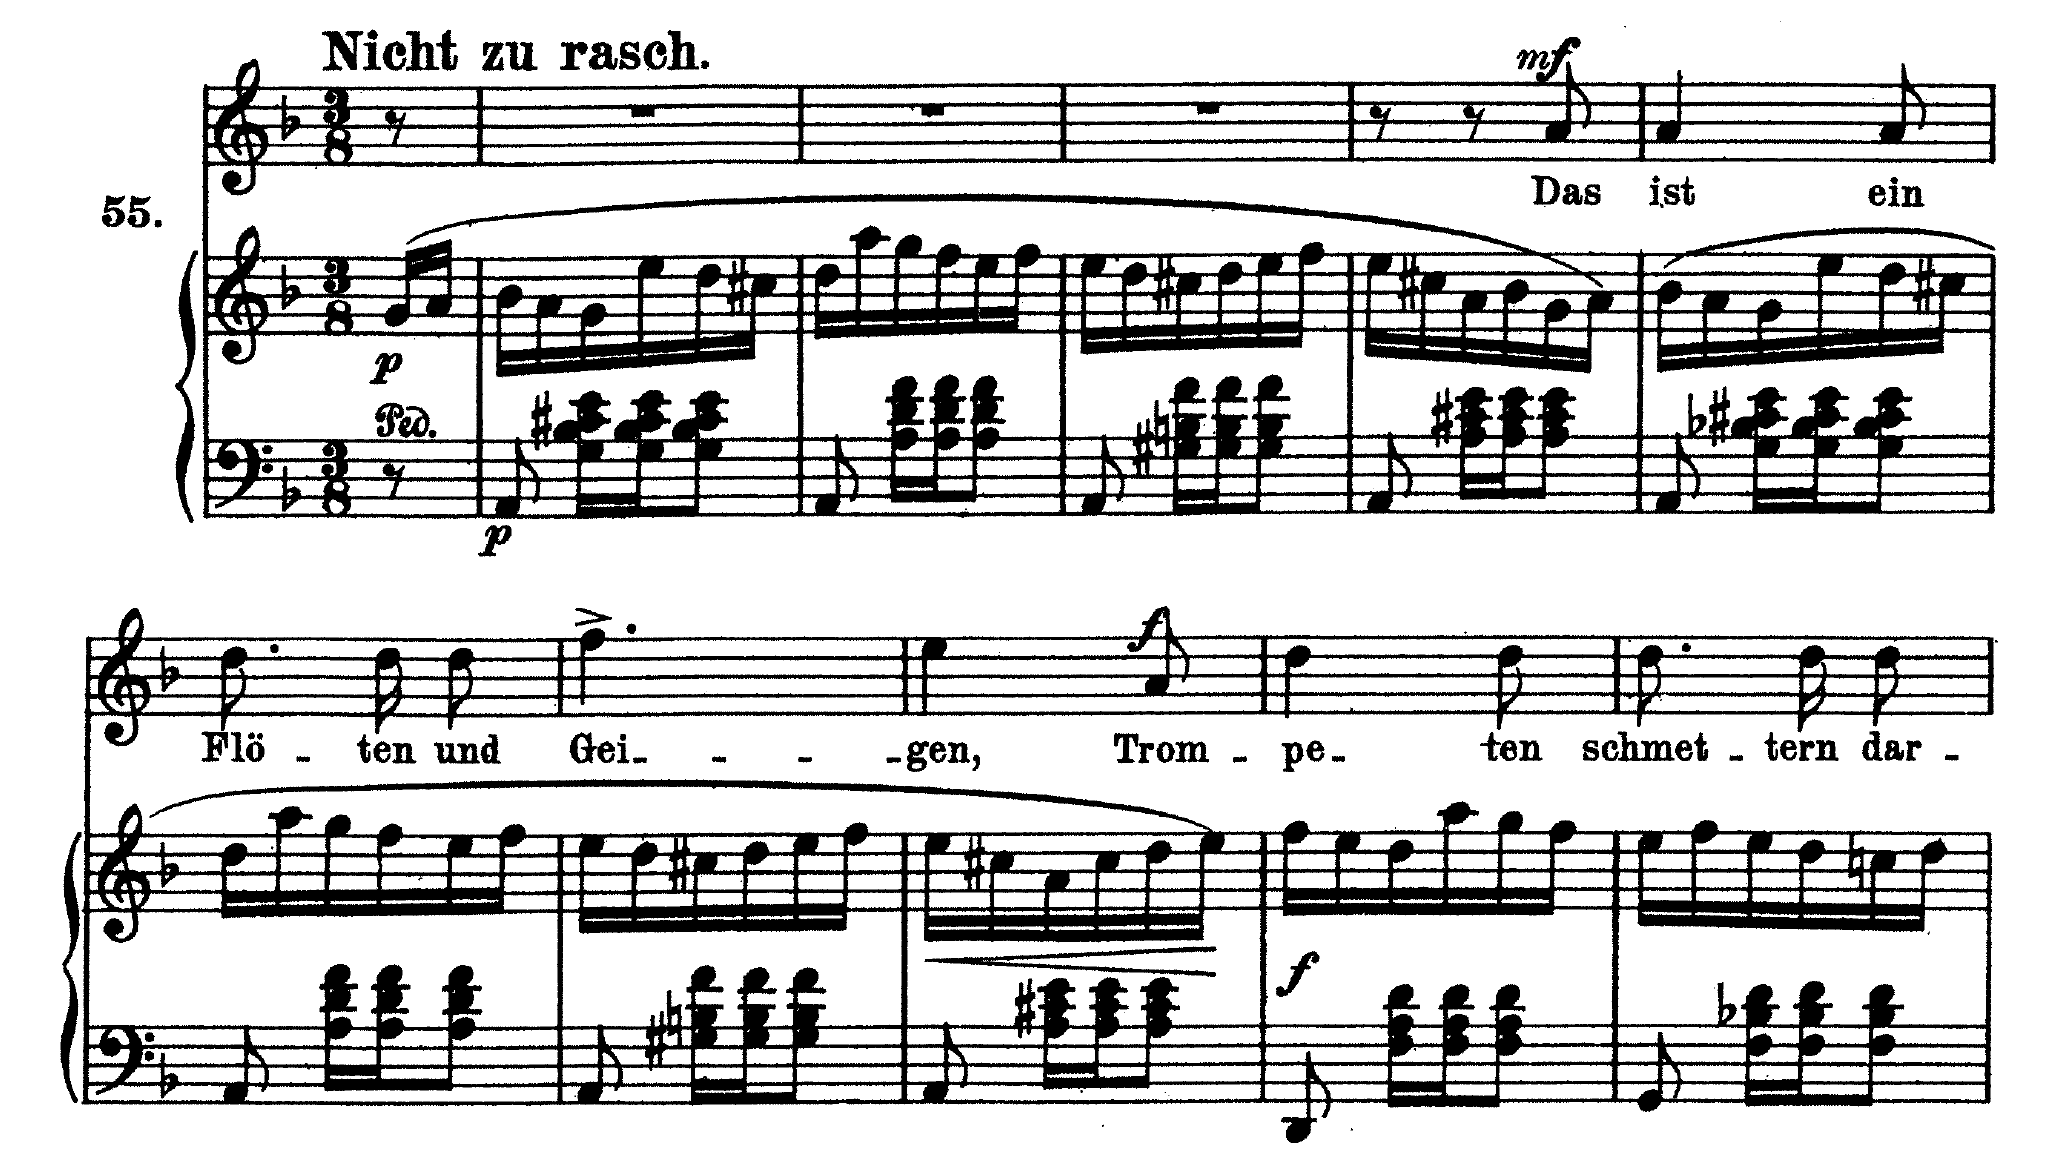
\includegraphics[width=0.7\linewidth]{giigen.png}
    \caption{The begining of "Das ist ein Flöten und Geigen"}
    \label{fig:enter-label}
\end{figure}
As analyzed earlier, irony dominates this text. Schumann's music also sounds ambiguous. Even the choice of key reveals the inner thoughts. At such a festive occasion, one would naturally expect a bright major key. But Schumann uses D minor (d-Moll) to present the beloved's wedding. D minor is far from the joy and charm of a wedding. The characteristic of D minor is mostly associated with melancholic and gloomy feelings or a mixture of sorrow with joy, often representing painful silent longing. The choice of a minor key for depicting the wedding is already full of irony, let alone the inherently ambiguous D minor, which exactly corresponds to the content of the poem.

Despite the melancholy key, this song is in a waltz-like 3/8 time, expressing the wedding dance. Musicologists call this rhythm a "grotesque ghost dance," which may seem exaggerated. But when looking more closely at the piano part, one can see that the chords of the left hand strike on an unaccented beat, creating a strange, distorted piano voice: what should be an elegant and joyful waltz thus sounds distorted and chaotic. In this sense, calling it a "ghost dance" is understandable. With this grotesque accompaniment, the right hand plays continuous sixteenth notes. There are almost no pauses between passages. One can easily imagine people spinning and spinning in a dance round without taking a break, which is very abnormal and unrealistic.

Some scholars describe this song as a "unique example of tone painting" because, in their view, "Against the wedding dance of the beloved, which the piano continuously continues to play, the voice of the rejected singer tries, as if to resist, in vain to assert itself." In fact, the singing voice is rather parallel to the piano voice than resistant. They seem independent of each other and not so closely connected, reflecting the booming at the wedding. Schumann himself marks accents on words like "dröhnen" (boom) and "stöhnen" (moan) in the notes, emphasizing the horror and disappointment of the lyrical "I".

As previously mentioned, Schumann himself added the word "wohl" (probably), seemingly to underscore the unrealistic aspect of the wedding. Upon closer examination of the notes, one can see that the first note in the singing voice is a dominant, creating an impression of instability. Furthermore, the last note in the singing voice remains on the subdominant and is not resolved. This is followed by a very long postlude. The famous English pianist and song accompanist Gerald Moore described this in his book \textit{Dichterliebe}: "He (Schumann) made his postludes more meaningful than the introductions. They possess luminous expression." This postlude also contains much information.\textsuperscript{\cite{ref2}} The key changes here from minor to major. The previously suppressed emotions suddenly break out, then become calmer and calmer, and the last bar ends in pianissimo. This dramatic ending is related to the added word "wohl", as if all the people dancing at the wedding gradually disappear and the lyrical "I" wakes up from its nightmare. This also creates a difference from Heine's original text: while the poet is completely horrified and desperate, the composer still holds on to the hope that everything is unreal until the end. Unlike the despair in Heine's text, Schumann's setting still clings to hope.
\begin{figure}[H]
    \centering
    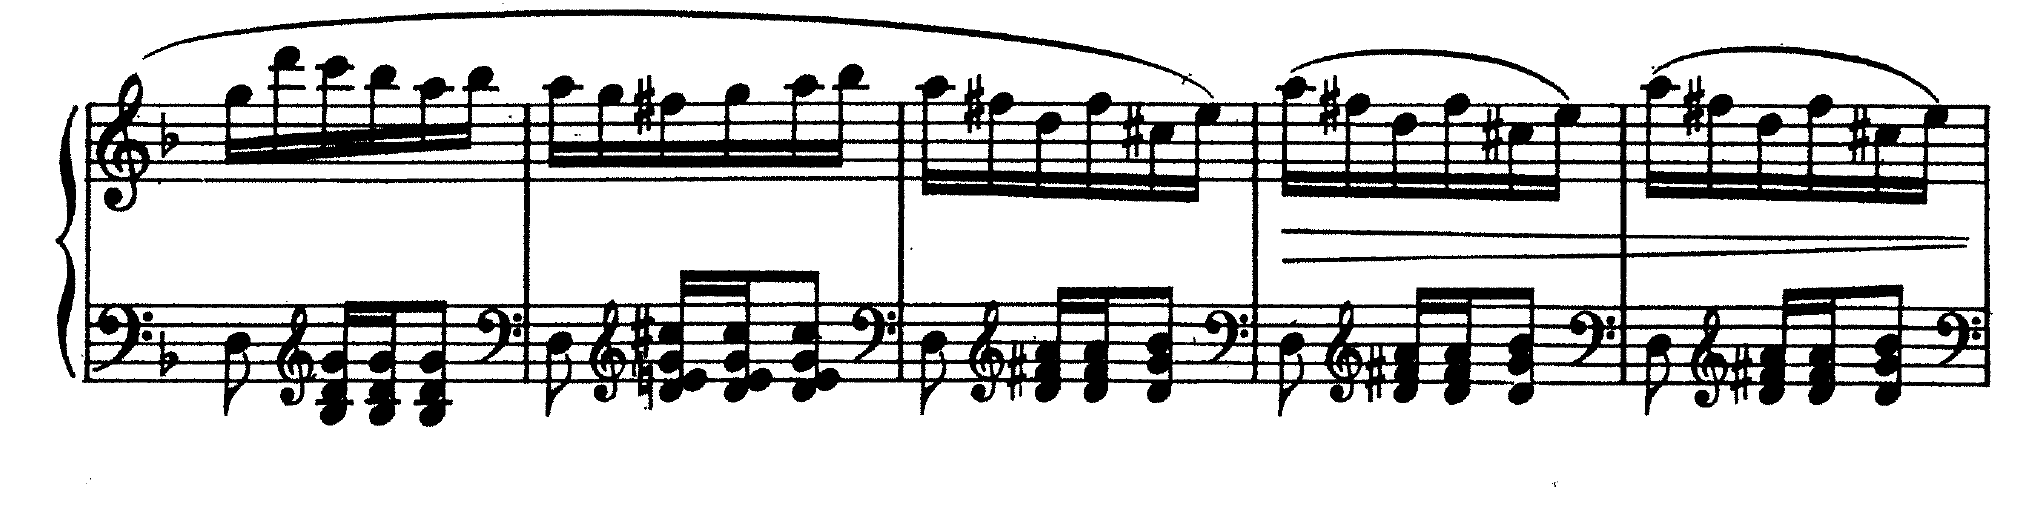
\includegraphics[width=0.7\linewidth]{piano melody.png}
    \caption{Melodies of Piano}
    \label{fig:}
\end{figure}
In summary, Schumann successfully incorporates such ironic elements into the music: the ironic choice of key, the contradictory rhythm, the parallel setting of the piano and singing voices, the deliberate accentuation—all serve as evidence. Text and music are closely intertwined. Nevertheless, the piano part plays a crucial role, especially in the postlude. Only through the piano voice does a dramatic and profound turn occur.

\section{Conclusion}
This essay is dedicated to analyzing the text-music relationship in the song cycle \textit{Dichterliebe} from the perspective of Heine's irony. The cycle was composed by Robert Schumann in 1840. The text is based on Heinrich Heine's \textit{Buch der Lieder}, specifically the section \textit{Lyrisches Intermezzo}.

Heine and Schumann are two great figures in literature and music, respectively, who play an important role at the intersection of these two disciplines. Heine, due to the particularly musical appeal of his texts, is one of the most frequently set poets in Germany. An examination of the text \textit{Lyrisches Intermezzo} reveals that the four-line stanzas, typically in trochaic or iambic meter, the metric musicality, the complex musical elements, the universality of the motifs, and the openness of the poem explain the particular attraction of this work for composers. At the same time, Romantic literature deeply influences Schumann. His dual talent in literature and music leads to a musical creation that is characteristic of him in music history. The dual characters “Florestan and Eusebius,” through whom he expresses his aesthetic conception, in a certain sense, approach Heine's literary views, which can be described as a focal point of Heine's irony. As a song composer, Schumann is marked by the selection of a text with high literary quality. Due to biographical similarities and aesthetic affinities, Schumann gradually turns to Heine's texts.

Schumann carefully selects and, in some cases, rearranges the 16 poems in \textit{Dichterliebe}, diverging from Heine's original order to create a coherent and suspenseful narrative. Apart from the dramaturgy of the cycle, Schumann also modifies the text in certain places when setting it to music. He changes words or adds his own. These modifications arise partly from musical considerations, but they also reflect his own literary thoughts.

Schumann employs various musical techniques to convey the ironic elements of the text in musical language. Firstly, the choice of key can have an ironic effect. Schumann uses a minor key to describe a wedding (“Das ist ein Flöten und Geigen,” op. 48/9). Schumann also effectively uses syncopation in appropriate places, as in “Das ist ein Flöten und Geigen” (op. 48/9), where the rhythmic contradiction underscores the abnormality of the situation. The tension in the text is musically presented through dissonance and modulation on certain words and phrases. Finally, the richly detailed postlude in the settings serves as an important aspect. The postlude acts as Schumann's reflection on Heine's text, containing dramatic turns and contrasting with the main part, similar to the punchline in Heine's works, elevating the irony to a new level.

"Hardly any composer of the 19th century has been celebrated by music historiography as a universal spirit of Romanticism as much as Robert Schumann," comments Sonja Gesse-Harm. In Schumann's \textit{Dichterliebe}, Friedrich Schlegel's poetic ideal seems to have been realized. Poetry and music are merged here. The song, in a certain sense, embodies Romantic poetry.
%----------------------------------------------------------

\printbibliography[title={REFERENCES}]

%----------------------------------------------------------

\end{document}